% !TeX root = ../main.tex

\section*{Density Estimation}
The task of density estimation is to obtain a continuous representation of the underlying pdf from a set of discrete samples (measurements). Note: that if we have the pdf we can do statistical analysis.

\begin{figure}[H]
  \centering
  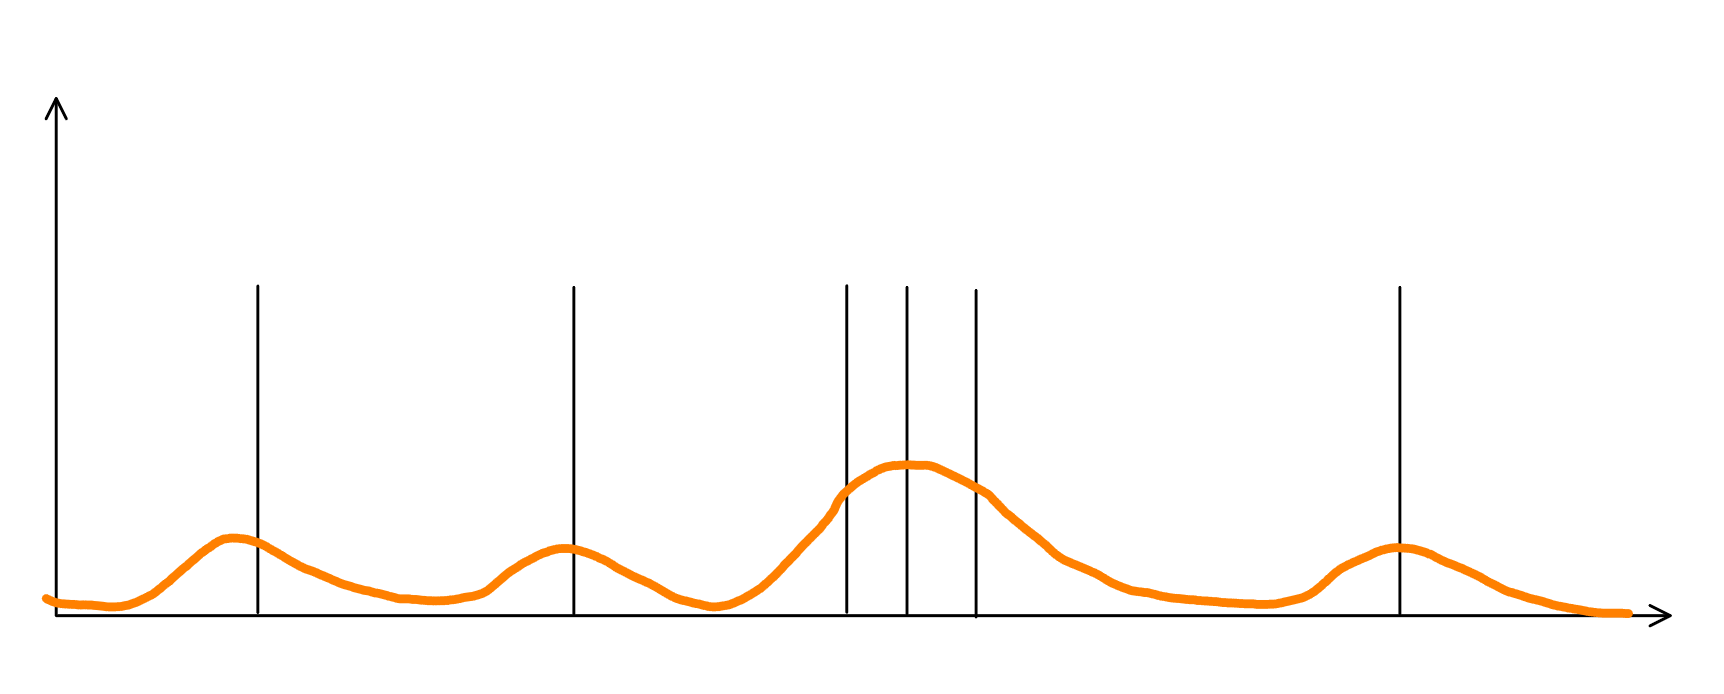
\includegraphics[width=0.6\textwidth]{01-pr-estimator}
  \caption{A PDF describing the distribution of measurements}
\end{figure}

Let $p(\vec{x})$ denote a probability density function pdf then:

\begin{enumerate}
  \item $p(\vec{x}) \ge 0$
  \item $\int_{-\infty}^\infty p(\vec{x}) \,d\vec{x} = 1$
  \item $p(\vec{a} \le \vec{x} \le \vec{b}) = \int_{\vec{a}}^{\vec{b}} p(\vec{x}) \,d\vec{x}$
\end{enumerate}

\paragraph{Parametric density estimation}
(mostly Pattern Recognition)

Make an assumption about the underlying distribution (e.g. Gaussian, GMM) and determine the best fitting distribution parameters from the data. (ML estimation, MAP estimation)

\paragraph{Non-parametric density estimation}

We make no assumption of the underlying Model. (Example Parzen-Rosenblatt estimator)

\paragraph{Sampling from a pdf}
Sampling provides a principle way of generating new / more data that behaves / looks similarly to the observations.

\begin{figure}[H]
  \centering
  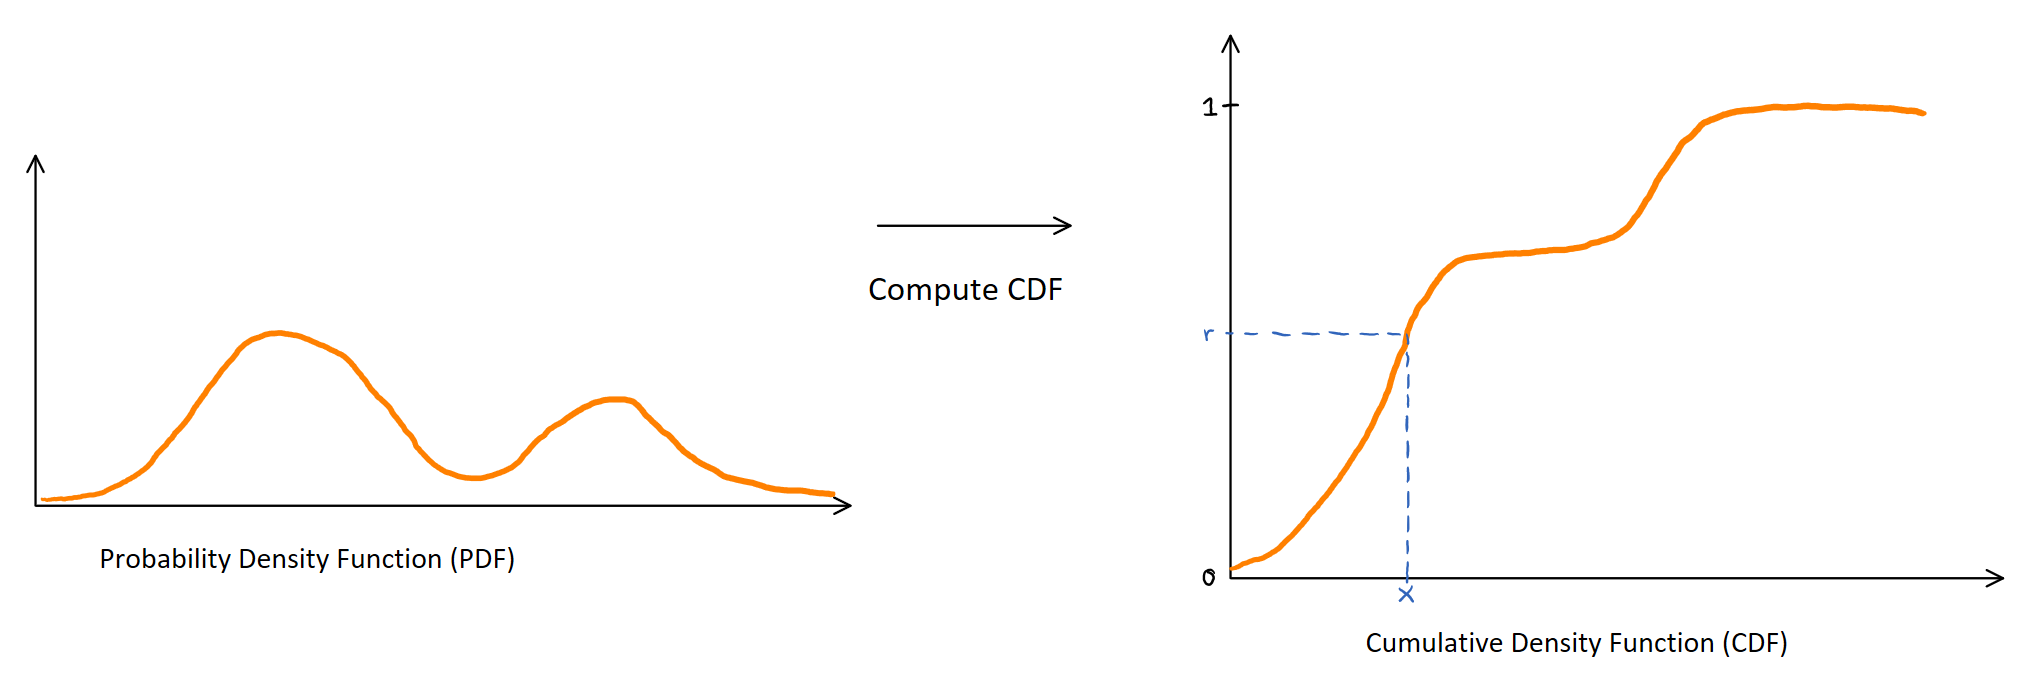
\includegraphics[width=0.9\textwidth]{02-pdf-cdf}
\end{figure}

Compute through discretization of the pdf $cdf[i] = cdf[i-1] + pdf[i]$. Then draw a uniformly distributed number ($r$) between 0 and 1. The sampled value is $x$ where $cdf[x] = r$.
